
\documentclass[sigconf,authordraft]{acmart}

%%
%% \BibTeX command to typeset BibTeX logo in the docs
\AtBeginDocument{%
  \providecommand\BibTeX{{%
    \normalfont B\kern-0.5em{\scshape i\kern-0.25em b}\kern-0.8em\TeX}}}

%%\setcopyright{acmcopyright}
%%\copyrightyear{2018}
%%\acmYear{2018}
%%\acmDOI{10.1145/1122445.1122456}

%% These commands are for a PROCEEDINGS abstract or paper.
%%\acmConference[Woodstock '18]{Woodstock '18: ACM Symposium on Neural
%%  Gaze Detection}{June 03--05, 2018}{Woodstock, NY}
%%\acmBooktitle{Woodstock '18: ACM Symposium on Neural Gaze Detection,
%%  June 03--05, 2018, Woodstock, NY}
%%\acmPrice{15.00}
%%\acmISBN{978-1-4503-9999-9/18/06}


%%
%% Submission ID.
%% Use this when submitting an article to a sponsored event. You'll
%% receive a unique submission ID from the organizers
%% of the event, and this ID should be used as the parameter to this command.
%%\acmSubmissionID{123-A56-BU3}

%%
%% The majority of ACM publications use numbered citations and
%% references.  The command \citestyle{authoryear} switches to the
%% "author year" style.
%%
%% If you are preparing content for an event
%% sponsored by ACM SIGGRAPH, you must use the "author year" style of
%% citations and references.
%% Uncommenting
%% the next command will enable that style.
%%\citestyle{acmauthoryear}

%%
%% end of the preamble, start of the body of the document source.
\begin{document}

%%
%% The "title" command has an optional parameter,
%% allowing the author to define a "short title" to be used in page headers.
\title{PAVE}

%%
%% The "author" command and its associated commands are used to define
%% the authors and their affiliations.
%% Of note is the shared affiliation of the first two authors, and the
%% "authornote" and "authornotemark" commands
%% used to denote shared contribution to the research.
\author{Samuel Leventhal}
%\authornote{Both authors contributed equally to this research.}
\email{samlev@cs.utah.edu}
\affiliation{%
  \institution{University of Utah School of Computing: Scientific Computing and Imaging Institute}
  %\streetaddress{P.O. Box 1212}
  %\city{Dublin}
  %\state{Ohio}
  %\postcode{43017-6221}
}
%\orcid{1234-5678-9012}
\author{Mark Kim}
\email{kimmb@ornl.gov}
\affiliation{%
  \institution{Oak Ridge National Lab}
  %\streetaddress{P.O. Box 1212}
  %\city{Dublin}
  %\state{Ohio}
  %\postcode{43017-6221}
}

\author{Dave Pugmire}
\authornotemark[1]
\email{pugmire@ornl.gov}
\affiliation{%
  \institution{Oak Ridge National Lab}}


%%
%% By default, the full list of authors will be used in the page
%% headers. Often, this list is too long, and will overlap
%% other information printed in the page headers. This command allows
%% the author to define a more concise list
%% of authors' names for this purpose.
\renewcommand{\shortauthors}{Leventhal and Kim, et al.}

%%
%% The abstract is a short summary of the work to be presented in the
%% article.
\begin{abstract}
  Science!
\end{abstract}

%%
%% The code below is generated by the tool at http://dl.acm.org/ccs.cfm.
%% Please copy and paste the code instead of the example below.
%%

\begin{CCSXML}
<ccs2012>
<concept>
<concept_id>10010405.10010432.10010439.10010440</concept_id>
<concept_desc>Applied computing~Computer-aided design</concept_desc>
<concept_significance>300</concept_significance>
</concept>
</ccs2012>
\end{CCSXML}

\ccsdesc[300]{Applied computing~Computer-aided design}

%%
%% Keywords. The author(s) should pick words that accurately describe
%% the work being presented. Separate the keywords with commas.
\keywords{VTKm, neural networks, generative adversarial network, Adios, PyTorch, path tracing}

%% A "teaser" image appears between the author and affiliation
%% information and the body of the document, and typically spans the
%% page.
\begin{teaserfigure}
  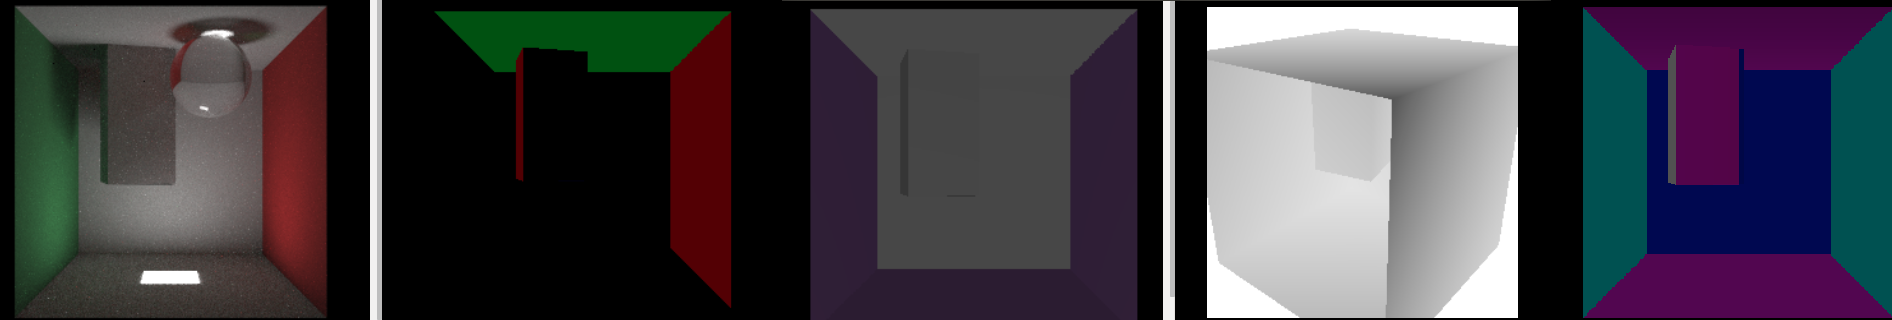
\includegraphics[width=\textwidth]{teaser}
  \caption{Rendered Conditional Images}
  \Description{Conditional Buffers and path traced rendered with VTKm to be used for training a PyTorch conditional generative adversarial network.}
  \label{fig:teaser}
\end{teaserfigure}

%%
%% This command processes the author and affiliation and title
%% information and builds the first part of the formatted document.
\maketitle
\section{Applicable ``Area of Interests'' Targets}
\begin{enumerate}
    \item In situ data management and infrastructures
Current Systems: production quality, research prototypes , Opportunities ,Gaps

Current Systems: integration of VTKm, Adios2 and Python (PyTorch). Prototype being a conditional generative adversarial network (cGAN) designed to use a VTKm based pathtracer applied but not limited to learning global illumination and light behavior in rendering tasks. 
Opportunities: Introducing a framework allowing researchers easy access to python on HPC systems as well as machine learning aided technique to treat and study experimental data used in scientific simulations as learnable probability distributions with derived conditional dependencies of interest.

   \item System resources, hardware, and emerging architectures.
Enabling Hardware, Hardware and architectures that provide opportunities for In situ processing, such as burst buffers, staging computations on I/O nodes, sharing cores within a node for both simulation and in situ processing

Enabling Hardware: By constructing an architecture allowing for Python to interface with VTKm data management controlled by Adios2 the proposed software allows for a well distributed simulation task among cores.

  \item Methods and algorithms:
Analysis: feature detection, statistical methods, temporal methods, geometric and topological methods 
Visualization: information visualization, scientific visualization, time-varying methods
  \item Case Studies and Data Sources
In situ methods/systems applied to data from simulations and/or experiments/observations
  \item Simulation and Workflows:
Integration:data modeling, software-engineering, 
Workflows for supporting complex in situ processing pipelines
  \item Requirements, Usability:
Reproducibility, provenance and metadata

\end{enumerate}

\section{Introduction}


\section{Related Work}

Tomas and Forbes Deep Illumination: \cite{deepillum}
VTKm \cite{vtkm}


\section{Motivation and Contribution}

\section{Implementation Design}

\section{Experiments}

\subsection{Cornell Box}
\subsection{Streamline Simulation}

\section{Results}

\section{Conclusions}



%%
%% The acknowledgments section is defined using the "acks" environment
%% (and NOT an unnumbered section). This ensures the proper
%% identification of the section in the article metadata, and the
%% consistent spelling of the heading.
\begin{acks}
Identification of funding sources and other support, and thanks to
individuals and groups that assisted in the research and the
preparation of the work should be included in an acknowledgment
section, which is placed just before the reference section in your
document.
\end{acks}

%%
%% The next two lines define the bibliography style to be used, and
%% the bibliography file.
\bibliographystyle{ACM-Reference-Format}
\bibliography{pave_ref}

%%
%% If your work has an appendix, this is the place to put it.
\appendix

\section{Appendix}



\end{document}
\endinput
%%
%% End of file `sample-authordraft.tex'.
